
\section{Rozbor problému}
\label{kap:1}

\subsection{SCARA}
\label{kap:1.1}

Scara robot je typ priemyselného robotického systému, ktorý bol vyvinutý na vykonávanie presných a opakujúcich sa úloh. Navrhol ho v roku 1979 vedec Hiroshi Makino z Yamanashi Univerzity\cite{}. Názov SCARA je akronym (Selective Compliance Assembly Robot Arm), ktorý značí, že vertikálna poddajnosť (compliance) je väčšia ako poddajnosť v horizontálnom smere. Najčastejšou úlohou je presun objektu z jedného miesta na druhé. Scara roboty majú zväčša 4 stupne voľnosti, a svojou konštrukciou pripomínajú ľudskú ruku(obr. \ref{OBRAZOK 1.1}).
\begin{figure}[h]
	\centering
	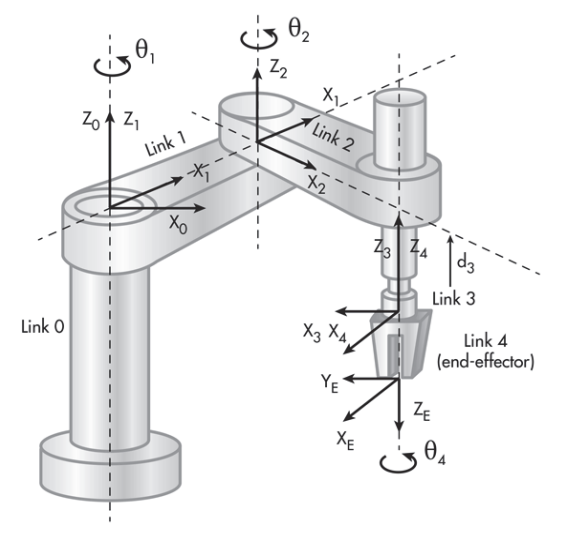
\includegraphics[width=100mm]{img/SCARA1.png}
	\caption{SCARA robot - smery pohybov\cite{}}\label{OBRAZOK 1.1} 
\end{figure} 
Ide o 3 rotačné a 1 posúvny kĺb, ktoré zabezpečujú pohyb robota vo všetkých osiach $x$, $y$ a $z$. Umiestneným otáčavých kĺbov v jednej rovine je pohyb robota v porovnaní s robotickými ramenami so 6 stupňami voľnosti, značne  znevýhodnený. Taktiež nosnosť týchto robotov je značne obmedzená, z dôvodu konštrukčných parametrov ako je nosnosť ložiska. Kinematická štruktúra SCARA robotov však prináša aj výhody, pre ktoré sú tieto roboty veľmi obľúbené a často používané.

Výhody:
\begin{itemize}
	\item   presnosť
	\item 	rýchlosť
	\item 	nízka hmotnosť
	\item   jednoduché ovládanie
	\item	menšie rozmery
	\item 	nižšia cena 
\end{itemize}

Tieto vlastnosti sú dôvodom prečo SCARA roboty nachádzajú široké uplatnenie a to hlavne v  montáži, balení, manipulácii s chemikáliami a oblastiach ako potravinárska výroba, laboratóriá, farmaceutický priemysel, automobilový priemysle atď.  

V tejto práci sa nebudeme venovať len klasickej štruktúre SCARA robota so 4 stupňami voľnosti ale budeme skúmať a overovať riešitelnosť daného problému aj pomocou iných kinematických štruktúr SCARA. Keďže posuvný pohyb z smere osi $z$ zabezpečuje dopravník, robot SCARA nepotrebuje posúvny kĺb, čím sa nám eliminuje 1 stupeň voľnosti. 
Z dôvodu zníženia ceny robota budeme tiež testovať, či je pre náš problém potrebný robot s 3 stupňami volnosti(3 rotačné kĺby) alebo vieme štruktúru ešte viacej zjednodušiť.   


\subsubsection{SCARA - 2 stupne voľnosti}
\label{kap:1.1.1}

Prvou testovanou štruktúrou bude SCARA s 2 rotačnými kĺbmi - 2 stupňe voľnosti. V tejto kinematickej štruktúre sa budú otáčať 2 ramená robota a nástroj na uchytenie objektu , ktorý sa nachádza na konci kinematického reťazca bude fixný.
Na obrázku \ref{OBRAZOK 1.1.1} môžeme vidieť model nášho ramena. Pri tejto konfigurácii je dôležité overiť na viacerých objektoch, rôznych tvarov a rozmerov, aké sú limitácie a schopnosti robota preniesť objekt zo štartovacej konfigurácie do cieľovej. Problém môže nastať hlavne pri väčších podlhovastých objektoch, kedy robot nebude vedieť v rámci svojich 2 rotácie ramien otočiť objekt do takej pozície aby dosiahol cieľovú konfiguráciu alebo nebude vedieť obísť stĺp na ktorom je rameno upevnené.  

\begin{figure}[h]
	\centering
	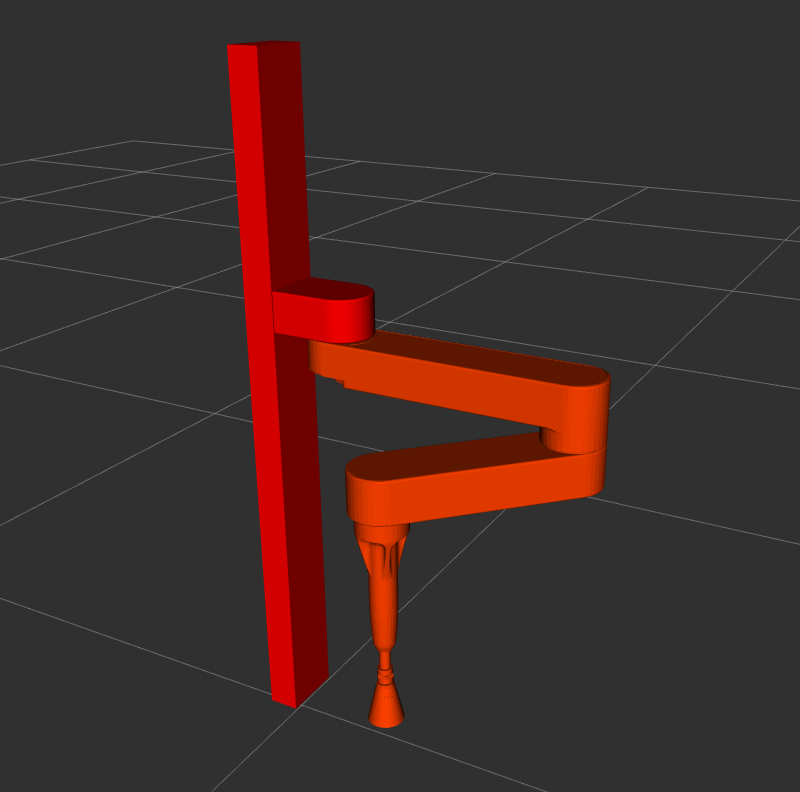
\includegraphics[width=80mm]{img/SCARA2.png}
	\caption{Model robota - Rviz}\label{OBRAZOK 1.1} 
\end{figure} 

\subsubsection{SCARA - 3 stupne voľnosti}
\label{kap:1.1.2}

Druhou štruktúrou, ktorú budeme testovať sa bude líšiť od prvej pridaním ďalšieho rotačného kĺbu, ktorý nám umožní otáčať nástrojom na uchytenie objektu. Pri tejto konfigurácii by mal byť robot schopný vždy nájsť trajektóriu na presun objektu zo štartu do cieľa. Tu budeme sledovať hlavne parametre a čas, za ktorý túto trajektóriu prejde a jej efektivitu. Tieto dáta budú potrebné na zhodnotenie, či je z hľadiska financií lepšie zvoliť väčšie náklady na efektívnejšieho robota v porovnaní s lacnejším robotom s väčšími obmedzeniami.

\subsection{Algoritmy plánovania trajektórie}
\label{kap:1.2}
Úloha plánovania trajektórie rohráva pri našom probléme veľkú rolu. Je potrebné zvoliť správny algoritmus aby sme vedeli dobre porovnať naše 2 kinematické štruktúry robota. 
\subsubsection{RRT}
\label{kap:1.2.1}

Algoritmus RRT – z anglického Rapidly-exploring Random Tree, by sa dal do slovenčiny preložiť ako rýchlo rastúci náhodný strom. Algoritmus je v oblasti robotiky veľmi rozšírení a obľúbený vďaka svojej schopnosti rýchlo prehľadávať vysoko dimenzionálny konfiguračný priestor, v ktorom zohľadňuje prekážky v priestore ako aj dynamiku telesa. \newline
Ide o algoritmus založený na prehľadávaní konfiguračného priestoru $C$ , kde sa v iteráciách vytvárajú náhodné uzly - $q$, ktorých spájaním vznikajú nové potenciálne cesty. Každý uzol $q$ reprezentuje pozíciu a orientáciu telesa v 2D alebo 3D priestore []. Pri plánovaní trajektórie je generovaný kontinuálny rad uzlov (obr. \ref{OBRAZOK 1.2.1}), ktorý začína v počiatočnom stave $q_{init}$,  a postupne sa rozrastá až dosiahne koncový stav $q_{goal}$.  Generovanie stromu prebieha v iteráciách kedy sa vždy vygeneruje náhodná konfigurácia $q_{rand}$ a nájde sa k nej najbližší uzol patriaci stromu. Od daného uzla je následne vo vzialenosti v od uzla $q_{nearest}$ vytvorený nový uzol $q_{new}$. Proces rozrastania stromu sa končí v momente ak sa $q_{new}$  nachádza v okolí cieľovej konfigurácie $q_{goal}$, ktoré je definované vzdialenosťou $d$. Ak neuvažujeme voľný konfiguračný priestor $C_{free}$ treba v procese generovania taktiež overovať kolíziu s danými prekážkami v priestore - $C_{obs}$. Novo generovaný uzol stromu sa nesmie nachádzať v priestore prekážky - $C_{obs}$, a ani cesta medzi dvoma susednými uzlami nesmie kolidovať s prekážkou. Pokiaľ uzol spĺňa tieto podmienky, je zaradený do štruktúry stromu, v opačnom prípade je vyradený a proces pokračuje ďalej.

\begin{figure}[h]
	\centering
	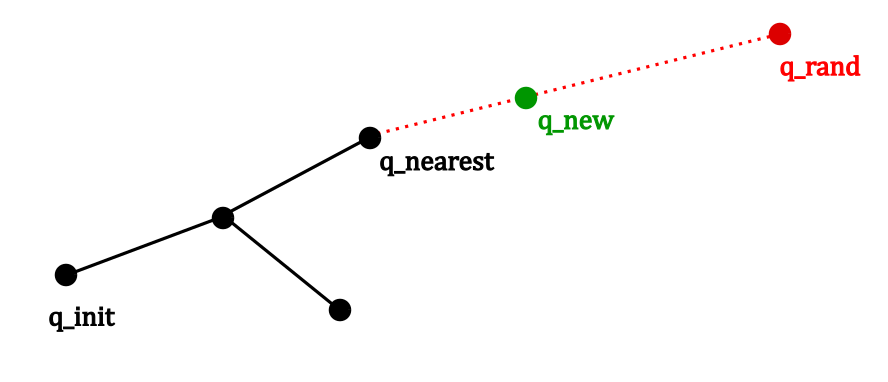
\includegraphics[width=120mm]{img/RRT1.png}
	\caption{Vizualizácia princípu RRT algoritmu }\label{OBRAZOK 1.2.1} 
\end{figure}  

Ide o neoptimálne riešenie, keďže body v konfiguračnom priestore sú generované náhodne a výsledný tvar trajektórie vzniká ako najkratšia cesta medzi nami vygenerovanými bodmi. Na zlepšenie trajektórie existuje viacero možností, ktoré ponúkajú suboptimálne riešenia problému, jedným z nich je napríklad RRT*.  

\subsubsection{RRT*}
\label{kap:1.2.2}

Jedná sa o modifikáciu RRT algoritmu, ktorej cieľom je v porovnaní s pôvodným RRT nájsť kratšiu trajektóriu. Hlavnou úpravou oproti jednoduchému RRT algoritmu je výpočet vzdialenosti z počiatočného do aktuálneho uzlu a následné overenie, či neexistuje v okolí uzol, ktorého vzdialenosť by bola menšia ako vzdialenosť momentálneho prepojenia. Ak táto situácia nastane, algoritmus vyberie prepojenie uzlov , ktoré vytvoria kratšiu trasu. Algoritmy sa tiež líšia ukončovacou podmienkou, kde pre RRT* je určený jasný počet iterácií. Od počtu iterácií závisí výsledný tvar trajektórie, kde so zvyšujúcim sa počtom je algoritmus schopný nájsť kratšie a plynulejšie trasy (obr. \ref{OBRAZOK 1.2.2}).

\begin{figure}[h]
	\centering
	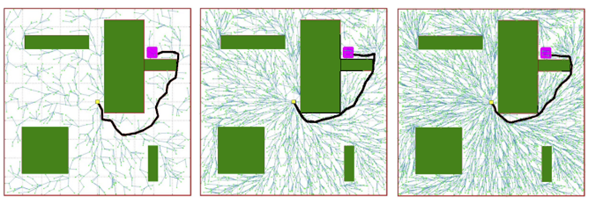
\includegraphics[width=160mm]{img/RRT2.png}
	\caption{Vplyv počtu iterácií na výslednú trajektóriu \cite{}}\label{OBRAZOK 1.2.2} 
\end{figure} 

\subsubsection{RRT - connect (prepojený)}
\label{kap:1.2.3}
Ďalšou z modifikácií je algoritmus RRT Connect (spojenie). Algoritmus v procese rozširovania stromovej štruktúry vytvára 2 stromy z počiatočnej a koncovej konfigurácie, ktoré sa šíria v konfiguračnom priestore až dokým nedôjde k ich spojeniu a tak vytvoreniu cesty (obr. \ref{OBRAZOK 1.2.3}). Výhodou tohoto algoritmu je fakt, že nájdenie trajektórie býva často lahšie dosiahnuteľný jedným z 2 možných smerov pohybu medzi dvoma bodmi, čo závisí od prekážok v priestore - $C_{obs}$. Použitím RRT - connect zvýšime pravdepodobnosť nájdenia trajektórie od počiatočného bodu ku koncovému.  

\begin{figure}[h]
	\centering
	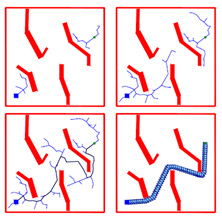
\includegraphics[width=70mm]{img/RRT-connect.png}
	\caption{Prepojenie 2 stromov \cite{}}\label{OBRAZOK 1.2.3} 
\end{figure} 

\subsubsection{Potenciálové pole}
\label{kap:1.2.4}

Plánovanie trajektórie na základe potenciálového poľa využíva koncept odpudivých a príťažlivých polí. Príťažlivé pole generuje veľmi nízke hodnoty so stredom v cieľovom bode, ktoré sa so zväčšujúcou sa vzdialenosťou od cieľa zvyšujú. Odpudivé pole zase naopak generuje veľmi vysoké hodnoty v okolí prekážok v priestore. Kombináciou daných dvoch polí dostávame tzv. potenciálové pole (obr. \ref{OBRAZOK 1.2.4}) so silným sklonom ku cieľu tak aby generovaná trajektória mala tendenciu vyhýbať sa prekážkam.

\begin{figure}[h]
	\centering
	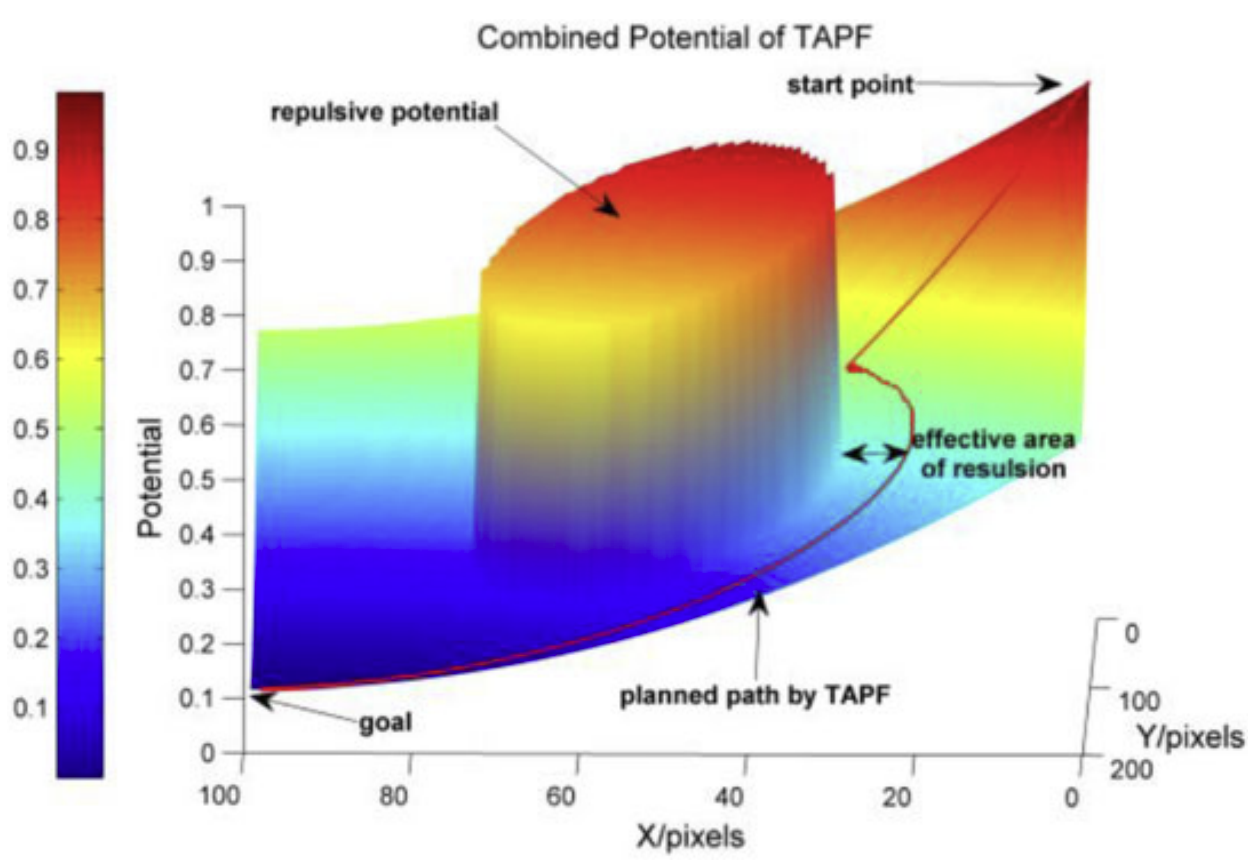
\includegraphics[width=100mm]{img/Potencialove_pole2.png}
	\caption{Potenciálové pole \cite{}}\label{OBRAZOK 1.2.4} 
\end{figure} 